% !TeX spellcheck = en_US
%\documentclass[10pt,a4paper,oneside]{book}
\documentclass[10pt,a4paper]{book}
\usepackage[utf8]{inputenc}
\usepackage{amsmath}
\usepackage{amsfonts}
\usepackage{amssymb}
\usepackage{makeidx}
\usepackage{graphicx}

% indent for first paragraph
\usepackage{indentfirst}

% deal with chapter titles
\usepackage{titlesec}
\titleformat{\chapter}
{\Large\bfseries} % format
{}                % label
{0pt}             % sep
{\huge}           % before-code


% set page margins
\usepackage[margin=1.2in]{geometry}

% set page margins
%\usepackage{anysize}
%\marginsize{3.0cm}{3.0cm}{3.0cm}{3.0cm}

% a garbage package you don't need except to create examples.
\usepackage{lipsum}

\usepackage{fancyhdr}
\pagestyle{fancy}
\lhead{This is my name}
\rhead{this is page \thepage}
\cfoot{center footer!}
\renewcommand{\headrulewidth}{0.4pt}
\renewcommand{\footrulewidth}{0.4pt}
% clear blank pages
\let\cleardoublepage\clearpage
% page n of m, usage:\thispagestyle{firststyle}
\fancypagestyle{firststyle}
{
	\fancyhf{}
	\fancyfoot[C]{\footnotesize Page \thepage\ of \pageref{LastPage}}
}

% footnote in footer, usage:\fancyfootnotetext{page_num}{this is the footnote}
\newcommand{\fancyfootnotetext}[2]{%
	\fancypagestyle{dingens}{%
		\fancyfoot[LO,RE]{\parbox{\textwidth}{\footnotemark[#1]\footnotesize #2}}%
	}%
	\thispagestyle{dingens}%
}

% set default typeface
\renewcommand*{\familydefault}{ppl}

% prevent floats from passing section
\usepackage[section]{placeins}

% support for Chinese. Note: UTF8 for pdflatex.
\usepackage[UTF8]{ctex}


% 目录索引超链接,放在最后
\usepackage[hidelinks]{hyperref}

\begin{document}

%\title{The Triangulation of Titling Data in
%	Non-Linear Gaussian Fashion via $\rho$ Series}
%\date{October 31, 475}
%
%\author{John Doe\thanks{Funded by NASA Grant \#42}}
%\maketitle

% 封面 turns off chapter numbering and uses roman numerals for page numbers
\frontmatter
% input partials
\begin{titlepage}
	\begin{center}
		
		% Upper part of the page. The '~' is needed because \\
		% only works if a paragraph has started.
		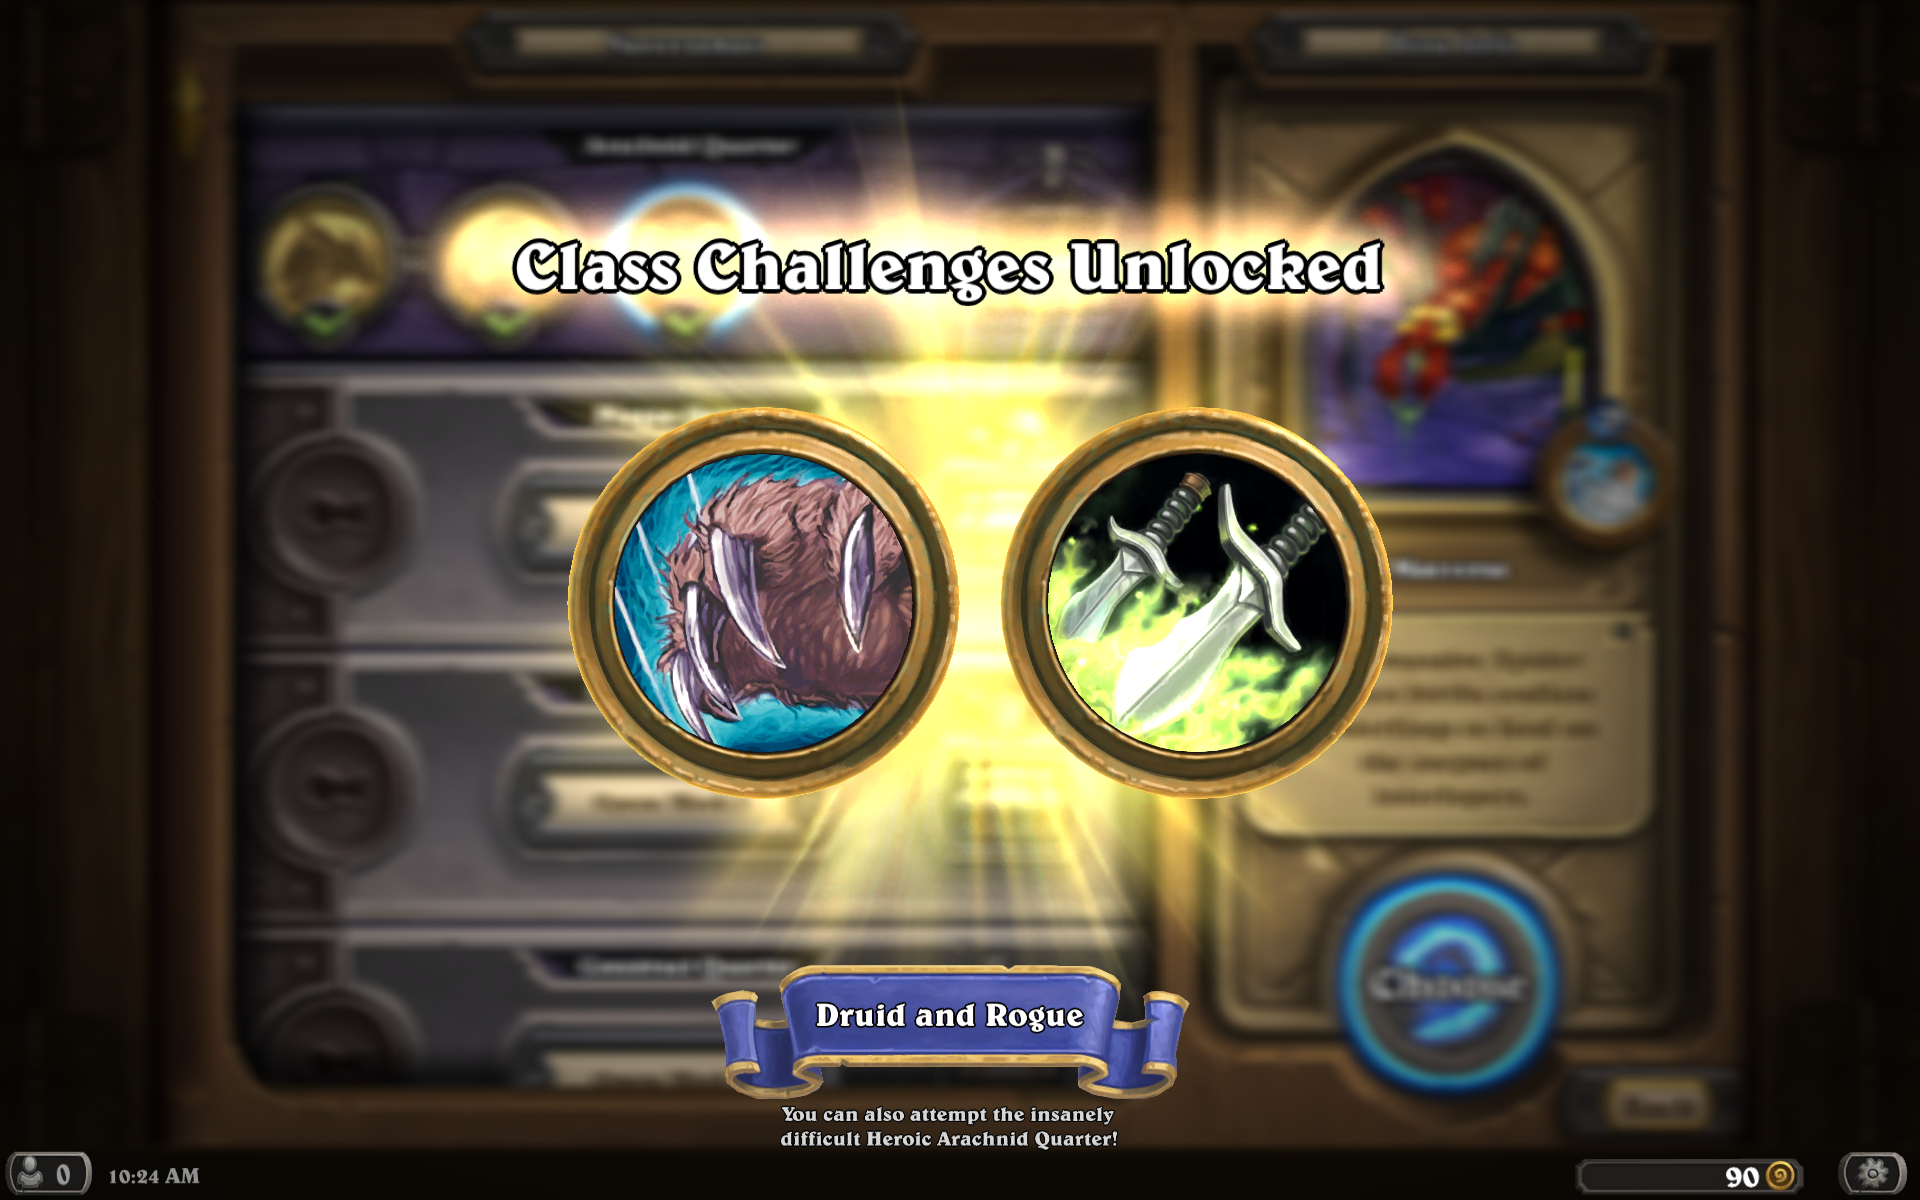
\includegraphics[width=0.6\textwidth]{graphics/hs}~\\[1cm]
		
		\textsc{\LARGE EVERTHIS.COM}\\[1.5cm]
		
		\textsc{\Large Final year project}\\[0.5cm]
		
		% Title
		\rule[1pt]{\textwidth}{2pt}
		{ \huge \bfseries Front end development \\[0.5cm] }
		
		\rule[10pt]{\textwidth}{2pt}
		
		% Author and supervisor
		\begin{minipage}{0.4\textwidth}
			\begin{flushleft} \large
				\emph{Author:}\\
				wwwap \textsc{everthis}
			\end{flushleft}
		\end{minipage}
		\begin{minipage}{0.4\textwidth}
			\begin{flushright} \large
				\emph{Supervisor:} \\
				Dr.~Mark \textsc{Brown}
			\end{flushright}
		\end{minipage}
		
		\vfill

		% Bottom of the page
		{\large \today}
		
	\end{center}

\end{titlepage}

% in two-side books, uncomment the line below. otherwise, comment it.
%\newgeometry{top=1in,bottom=1in,right=0.5in,left=1.5in}

% 目录
\tableofcontents

% turns on chapter numbering, resets page numbering and uses arabic numerals for page numbers
\mainmatter

%  resets chapter numbering, uses letters for chapter numbers and doesn't fiddle with page numbering
%\appendix

% turns off chapter numbering and doesn't fiddle with page numbering.
%\backmatter

\chapter{chapter first}
\section{section01}
\paragraph{测试}
一千九百八十年间,西京城里出了桩异事,两个关系是死死的朋友,一日活得泼烦一千九百八十年间,西京城里出了桩异事,两个关系是死死的朋友,一日活得泼烦一千九百八十年间,西京城里出了桩异事,两个关系是死死的朋友,一日活得泼烦一千九百八十年间,西京城里出了桩异事,两个关系是死死的朋友,一日活得泼烦一千九百八十年间,西京城里出了桩异事,两个关系是死死的朋友,一日活得泼烦一千九百八十年间,西京城里出了桩异事,两个关系是死死的朋友,一日活得泼烦一千九百八十年间,西京城里出了桩异事,两个关系是死死的朋友,一日活得泼烦一千九百八十年间,西京城里出了桩异事,两个关系是死死的朋友,一日活得泼烦一千九百八十年间,西京城里出了桩异事,两个关系是死死的朋友,一日活得泼烦一千九百八十年间,西京城里出了桩异事,两个关系是死死的朋友,一日活得泼烦一千九百八十年间,西京城里出了桩异事,两个关系是死死的朋友,一日活得泼烦一千九百八十年间,西京城里出了桩异事,两个关系是死死的朋友,一日活得泼烦一千九百八十年间,西京城里出了桩异事,两个关系是死死的朋友,一日活得泼烦一千九百八十年间,西京城里出了桩异事,两个关系是死死的朋友,一日活得泼烦一千九百八十年间,西京城里出了桩异事,两个关系是死死的朋友,一日活得泼烦一千九百八十年间,西京城里出了桩异事,两个关系是死死的朋友,一日活得泼烦一千九百八十年间,西京城里出了桩异事,两个关系是死死的朋友,一日活得泼烦一千九百八十年间,西京城里出了桩异事,两个关系是死死的朋友,一日活得泼烦一千九百八十年间,西京城里出了桩异事,两个关系是死死的朋友,一日活得泼烦一千九百八十年间,西京城里出了桩异事,两个关系是死死的朋友,一日活得泼烦一千九百八十年间,西京城里出了桩异事,两个关系是死死的朋友,一日活得泼烦一千九百八十年间,西京城里出了桩异事,两个关系是死死的朋友,一日活得泼烦一千九百八十年间,西京城里出了桩异事,两个关系是死死的朋友,一日活得泼烦一千九百八十年间,西京城里出了桩异事,两个关系是死死的朋友,一日活得泼烦一千九百八十年间,西京城里出了桩异事,两个关系是死死的朋友,一日活得泼烦一千九百八十年间,西京城里出了桩异事,两个关系是死死的朋友,一日活得泼烦一千九百八十年间,西京城里出了桩异事,两个关系是死死的朋友,一日活得泼烦一千九百八十年间,西京城里出了桩异事,两个关系是死死的朋友,一日活得泼烦一千九百八十年间,西京城里出了桩异事,两个关系是死死的朋友,一日活得泼烦一千九百八十年间,西京城里出了桩异事,两个关系是死死的朋友,一日活得泼烦一千九百八十年间,西京城里出了桩异事,两个关系是死死的朋友,一日活得泼烦一千九百八十年间,西京城里出了桩异事,两个关系是死死的朋友,一日活得泼烦一千九百八十年间,西京城里出了桩异事,两个关系是死死的朋友,一日活得泼烦一千九百八十年间,西京城里出了桩异事,两个关系是死死的朋友,一日活得泼烦一千九百八十年间,西京城里出了桩异事,两个关系是死死的朋友,一日活得泼烦一千九百八十年间,西京城里出了桩异事,两个关系是死死的朋友,一日活得泼烦一千九百八十年间,西京城里出了桩异事,两个关系是死死的朋友,一日活得泼烦一千九百八十年间,西京城里出了桩异事,两个关系是死死的朋友,一日活得泼烦一千九百八十年间,西京城里出了桩异事,两个关系是死死的朋友,一日活得泼烦一千九百八十年间,西京城里出了桩异事,两个关系是死死的朋友,一日活得泼烦一千九百八十年间,西京城里出了桩异事,两个关系是死死的朋友,一日活得泼烦一千九百八十年间,西京城里出了桩异事,两个关系是死死的朋友,一日活得泼烦一千九百八十年间,西京城里出了桩异事,两个关系是死死的朋友,一日活得泼烦一千九百八十年间,西京城里出了桩异事,两个关系是死死的朋友,一日活得泼烦一千九百八十年间,西京城里出了桩异事,两个关系是死死的朋友,一日活得泼烦。

\chapter{chapter second}
\section{section02}
\begin{figure}
	\centering
	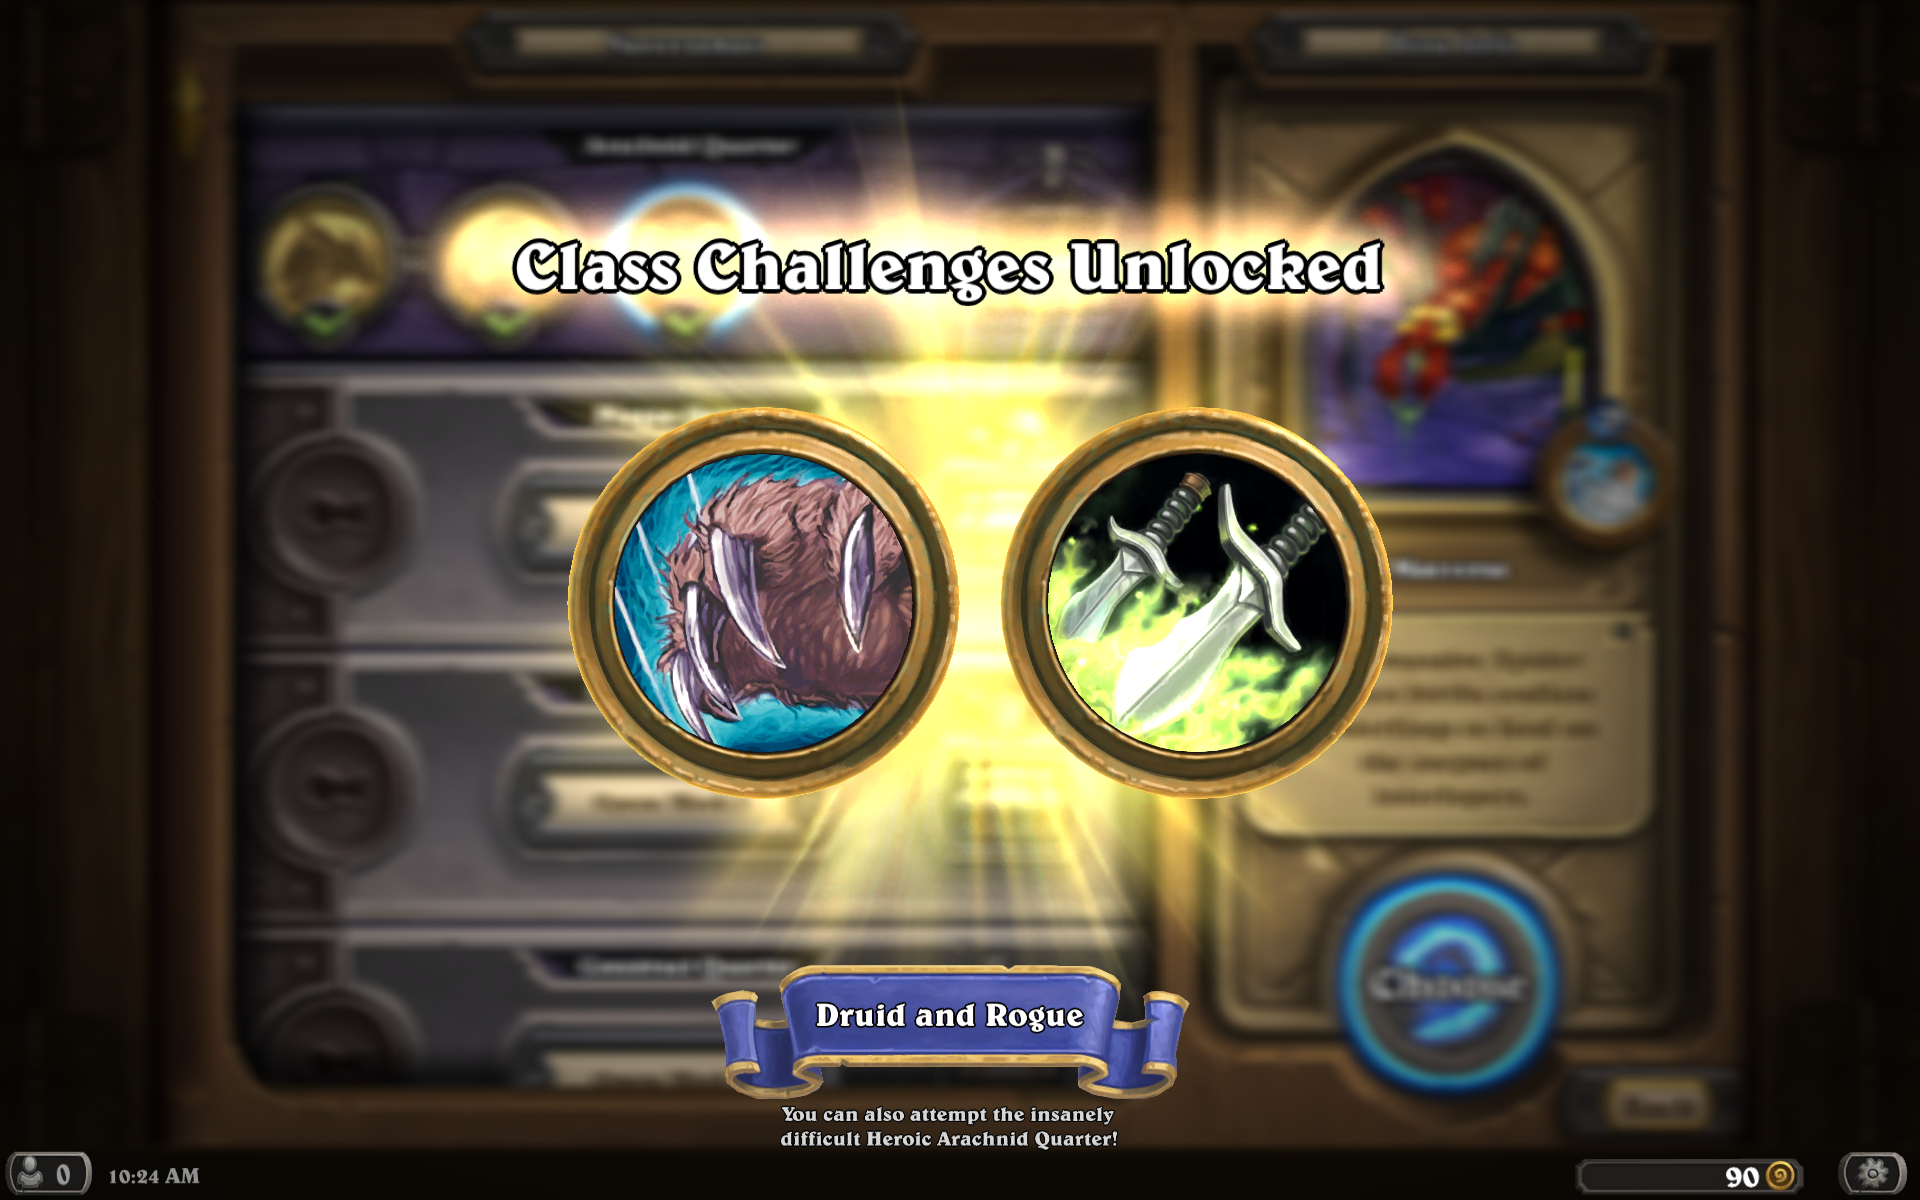
\includegraphics[width=0.7\textwidth,natwidth=1920,natheight=1200]{graphics/hs}
	\caption{hejdkaljdla}
	\label{fig:hs}
\end{figure}
\lipsum[1-2]
\section{section03}

\chapter{中文测试}
滑动断过的嘎目录索引超链接,放在最后\footnotemark[1]
\fancyfootnotetext{1}{this is the footnote}

\end{document}
